\documentclass[a4paper]{jpconf}
\usepackage{graphicx}
\usepackage{color}
\usepackage{array}
\newcommand{\cred}[1]{{\color{red}#1}}

\begin{document}
\title{Vibrational characteristics of a superconducting magnetic bearing employed for a prototype polarization modulator}

\author{Yuki Sakurai$^{1}$, Tomotake Matsumura$^{1}$, Hajime Sugai$^{1}$, Nobuhiko Katayama$^{1}$, Hiroyuki Ohsaki$^{2}$, Yutaka Terao$^{2}$, Yusuke Terachi$^{2}$, Hirokazu Kataza$^{3}$, Shin Utsunomiya$^{1}$, Ryo Yamamoto$^{3}$}
\vspace{2mm}
\address{
$^{1}$Kavli Institute for the Physics and Mathematics of the Universe (WPI),The University of Tokyo Institutes for Advanced Study, The University of Tokyo, 5-1-5 Kashiwanoha, Kashiwa, Chiba 277-8583, Japan \\
$^{2}$Graduate School of Frontier Sciences, The University of Tokyo, 5-1-5 Kashiwanoha, Kashiwa, Chiba 277-8561, Japan \\
$^{3}$Japan Aerospace Exploration Agency, Institute of Space and Astronautical Science (ISAS), 3-1-1 Yoshinodai, Chuo-ku, Sagamihara, Kanagawa 252-5210, Japan
}

\ead{yuki.sakurai@ipmu.jp, tomotake.matsumura@ipmu.jp}

\begin{abstract}
We present the vibrational characteristics of a levitating rotor in a superconducting magnetic bearing (SMB) system operating at below 10 K.
We develop a polarization modulator that requires a continuously rotating optical element, called half-wave plate (HWP), for a cosmic microwave background polarization experiment.
The HWP has to operate at the temperature below 10 K, and thus an SMB provides a smooth rotation of the HWP at the cryogenic temperature at about 10K with minimal heat dissipation.
In order to understand the potential interference to the cosmological observations due to the vibration of the HWP,
it is essential to characterize the vibrational properties of the levitating rotor of the SMB.
We constructed a prototype model that consists of an SMB with an array of high temperature superconductors, YBCO, and a permanent magnet ring.
The rotor position is monitored by the laser displacement gauge, and the cryogenic Hall sensor via the magnetic field.
In this presentation, we present the measurement results of the vibration characteristics using our prototype SMB system.
We discuss the spring constant and the magnetic field inhomogeneity of the SMB and sub-components including a rotation frequency monitoring system, a holder mechanism, and drive system.
Finally, we discuss the projected performance of this technology toward the use in future space missions.
\end{abstract}

\section*{Introduction}

A cosmic microwave background (CMB) is electromagnetic microwave radiation from the big bang of the universe.
It is still observable isotropically in whole sky today.
One of most important research topics in the current cosmology and high-energy physics is to study the cosmic inflation theory, which predicts a rapid expansion of the universe after $\sim 10^{-38}$ seconds from the beginning of the universe~\cite{inflation_sato,inflation_guth}.
The inflation solves several mysteries of the standard cosmology and it can provide a foothold for new physics in high energy physics.
The theory predicts that the inflation left the divergence free pattern in the CMB polarization,  called "B-mode".
Therefore, the experimental discovery of the cosmic inflation is possible by observing the CMB B-mode polarization.
A world-wide keen discovery race is spreading among many CMB polarization experiments.
Along with that, the instrumental development has progressed remarkably.

One of the critical instruments for a precise measurement of the CMB polarization is a "polarization modulator".
It consists of an optical element, a half-wave plate (HWP), and a rotational mechanism.
The continuously rotating HWP modulates the CMB polarization signal synchronously at the four times of the rotational frequency of the HWP, a few Hz.
%Since the intrinsic instrumental noise is not modulated, systematic uncertainties are significantly reduced.
On the other hand, the continuously rotating HWP have to be maintained at cryogenic temperature ($\sim$ 10~K) in order to reduce the detector noise originating from the thermal emission of the HWP itself.
It is therefore necessary to use a rotational mechanism which allows to rotate with minimal heat dissipation at cryogenic temperature.

In general mechanical bearings, there is too much frictional heat due to physical contact.
Thus, a superconducting magnetic bearing (SMB) is a good candidate for the rotational mechanism~\cite{smb}.
The SMB is a rotational bearing utilizing magnetic levitation by the type II superconductor and the magnetic field from a permanent magnet, and thus there is no physical contact between a rotor and a stator.
\cred{tomo: continue editing from here}It is possible to achieve minimal heat dissipation at cryogenic temperature with the SMB.
The SMB is developed mainly for industries such as flywheel energy storage,
although the polarization modulator is one of unique applications and it plays critical role in the CMB polarization experiments.
A balloon experiment called EBEX has succeeded the CMB polarization observation with the polarization modulator employing the SMB system \cite{ebex}.
Currently, the CMB polarization experiments which consider to implements this system are increasing on the ground and even on the satellites \cite{litebird}.

For the polarization modulator, the SMB system has advantages in terms of heat.
However, it is also necessary to consider the deviation of the optical axis of the HWP related to the stiffness of the SMB.
We evaluate this stiffnes as a spring constant since the dynamics of the electromagnetic force of the SMB system can be analogied as a spring system.

In this paper, we describe the result of the vibration measurement of the SMB of 384~mm diameter.
Since the typical aperture size of a CMB telescope is 400~mm, so that this diameter (D=384~mm) is close to an actual application.

\section*{Experimental Setup}


We conducted vibration measurment using a Styro- foam bucket with liquid nitrogen as shown in Figure \ref{fig:d400}.
Although the SMB system is operated inside the 4~K cryostat in an actual CMB observation, a liquid nitrogen temperature (77~K) is sufficient for the vibration measurement.

We prepare the SMB system with inner diameter of 384~mm.
Due to the relatively large diameter, The ring shaped magnet, which consists of 16 segmented NdFeB magnets, are used as the rotor magnet.
Each segmented magnet is magnetized axially with the magnetic remnance of 1.24 T.
A YBa$_{2}$Cu$_{3}$O$_{\mathrm{x}}$ (YBCO) superconductor is used as the stator, which is one of High Temperature Superconductors and its transision temperature is $\sim$ 95~K.
The YBCO array is formed in a ring shape using three-seeded YBCO tiles.
The NdFeB ring magnet and the YBCO array are fabricated by Adelwitz Technologiezentrum GmbH (ATZ) company in Germany \cite{ATZ}.
The YBCO array is submerged by the liquid nitrogen but the rotor mganet is exposed to the room environment.
We set a space between the rotor magnet and YBCO array with aluminum plates at room temperature enviroment, and then a liquid nitrogen was poured.
After the temperature of the YBCO array becomes below its transition temperature, the plates are removed for magnetic levitation.
The levitation height, defined as the distance between the bottom of the rotor magnet and the top of the YBCO array, is controled by the tickness of the aluminum plate.
We measure the rotor vibration in the axial direction with four different levitation heights (3~mm, 6~mm, 9~mm and 12~mm).
In order to enhance the vibration amplitude, an external impulse force was applied by hand in the axial direction.

The displacement of the rotor is monitored by a laser displacement gauge (keyence LK-500),
which is mounted by an aluminum frame jig at a distance of 260 mm from the top of the rotor magnet as shown in Figure \ref{fig:d400}.
Since The displacement of the rotor magnet due to the vibration also affects the magnetic field,
we also measure the magnetic field by a Hall sensor mounted at the top surface of the YBCO array.

\begin{figure}[htbp]
  \centering
  \begin{minipage}{0.6\hsize}
    \includegraphics[width=85mm]{D400mm.eps}
    \caption{The experimental setup for the vibration measurements for $D=384$~mm}
    \label{fig:d400}
  \end{minipage}
  \begin{minipage}{0.3\hsize}
    \centering
    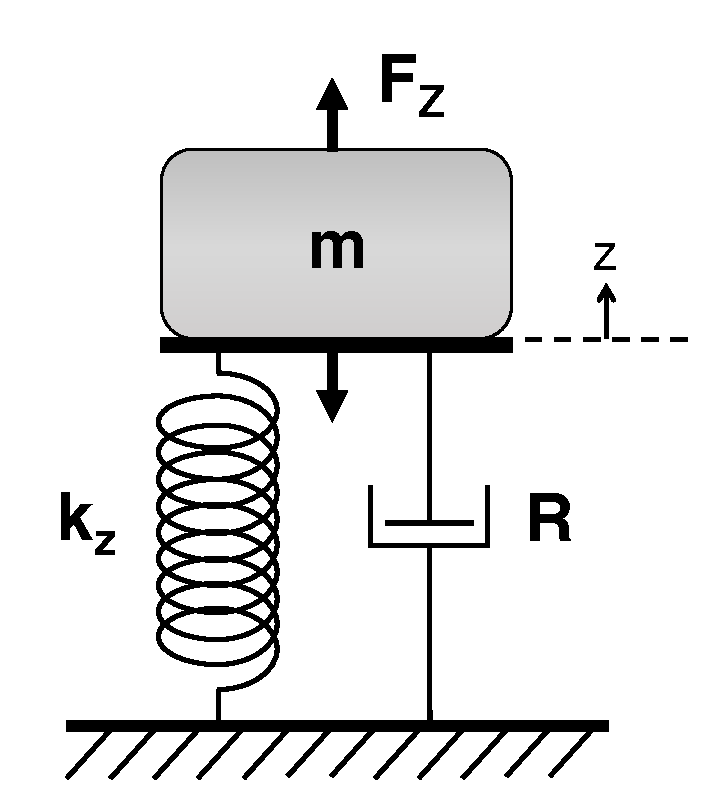
\includegraphics[width=50mm]{SpringSystem.eps}
    \caption{Mass-Spring-Damper model}
    \label{fig:msd}
  \end{minipage}
\end{figure}


\section*{Result and Discussion}

An axial vibration of the rotor can be descrived by a damping motion of a mass-spring-damper model shown in Figure \ref{fig:msd}.
The motion of this model is expressed by
\begin{equation}
  m \frac{\partial^{2} x}{\partial^{2} t} + R \frac{\partial x}{\partial t} + k_{z} x = 0,
  \label{eq:damping_motion}
\end{equation}
where $m$ is the mass of the rotor (3.0~kg), $R$ is the damping coefficient and $k_{z}$ is the spring constant.
Under the condition of the damping motion, the solution of the equation (\ref{eq:damping_motion}) is
\begin{equation}
  x = A \mathrm{e}^{- \zeta \omega_{0} t} \cos( \sqrt{1 - \zeta^{2}} \ \omega_{0} t + \phi),
  \label{eq:damping}
\end{equation}
where $\zeta = R / 2 \sqrt{mk_{z}}$ is the damping ratio and $\omega_{0} = \sqrt{k_{z}/m}$ is the undamped angular frequency.
The parameters of $A$ and $\phi$ are the amplitude and the phase determind by the magnitude and timing of the external impulse force.
Thus, these values are changed every time.

Figure \ref{fig:vibration_up} shows the laser gauge output and the Hall sensor output as a function of time at the levitation hegith of 9~mm.
We fit the data with equation (\ref{eq:damping}) and derive the unknwon parameters of $\zeta$ and $\omega_{0}$ for each leviration height.
The fitting result of the Hall sensor output with the levitation height of 12~mm is shown the right plot of Figure \ref{fig:vibration}.
The fitted parameters are summarized in Table \ref{tab:fit_result}.
The parameters between the laser gauge and the Hall sensor are consistent within 10~\%.

\renewcommand{\arraystretch}{1.2}
\begin{table}[htbp]
  \centering
  \newcolumntype{Y}{>{\centering\arraybackslash}p{18mm}}
  \begin{tabular}{c|YYYY}
    \hline
    & \multicolumn{4}{c}{Laser gauge} \\
    h [mm] & $\zeta$  & $\omega_{0}$ [rad/s] & $R$ [N$\cdot$s/m] & $k_{z}$ [Nm] \\ \hline
    3  & 2.1$\times10^{-2}$ & 331.8 & 42.0 & 3.3$\times10^{5}$ \\
    6  & 2.7$\times10^{-2}$ & 194.0 & 31.0 & 1.1$\times10^{5}$ \\
    9  & 2.3$\times10^{-2}$ & 138.2 & 19.1 & 5.7$\times10^{4}$ \\
    12 & 1.8$\times10^{-2}$ & 111.7 & 11.8 & 3.7$\times10^{4}$ \\
    \hline
    & \multicolumn{4}{c}{Hall sensor} \\
    h [mm] & $\zeta$  & $\omega_{0}$ [rad/s] & $R$ [N$\cdot$s/m] & $k_{z}$ [Nm] \\ \hline
    3  & 2.4$\times10^{-2}$ & 299.3 & 43.5 & 2.7$\times10^{5}$ \\
    6  & 2.3$\times10^{-2}$ & 195.7 & 27.1 & 1.2$\times10^{5}$ \\
    9  & 2.4$\times10^{-2}$ & 136.4 & 20.2 & 5.6$\times10^{4}$ \\
    12 & 2.4$\times10^{-2}$ & 108.0 & 15.7 & 3.5$\times10^{4}$ \\
    \hline

  \end{tabular}
  \caption{The summary of the fit parameters from the vibration measurements. h is the levitation height. $\zeta$ and $\omega_{0}$ is the damping ratio and undamped angular frequency.
    $R$ is the damping coefficient and $k_{z}$ is the spring constant.
    \label{tab:fit_result}}
\end{table}
\renewcommand{\arraystretch}{1.0}

We also apply a Fourier transformation for the data of the Hall sensor output.


blah blah blah


\begin{figure}[htbp]
  \centering
  \begin{minipage}{0.45\hsize}
  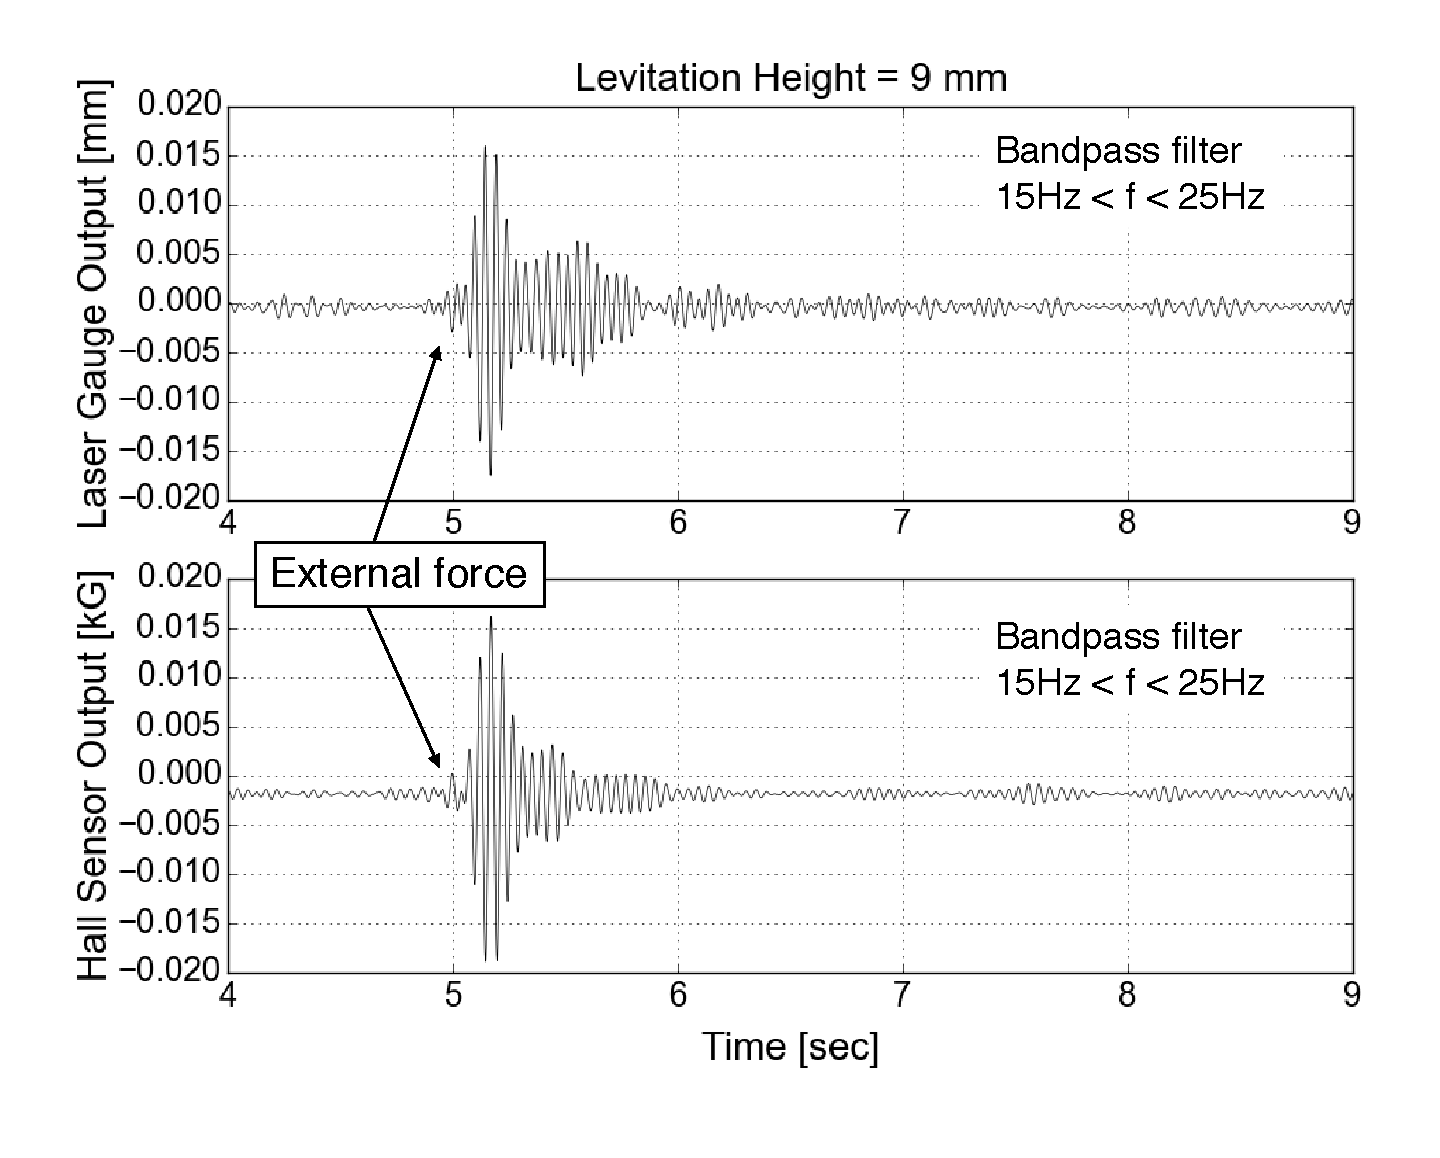
\includegraphics[width=70mm]{vibration_up.eps}
  \end{minipage}
  \begin{minipage}{0.45\hsize}
    \centering
    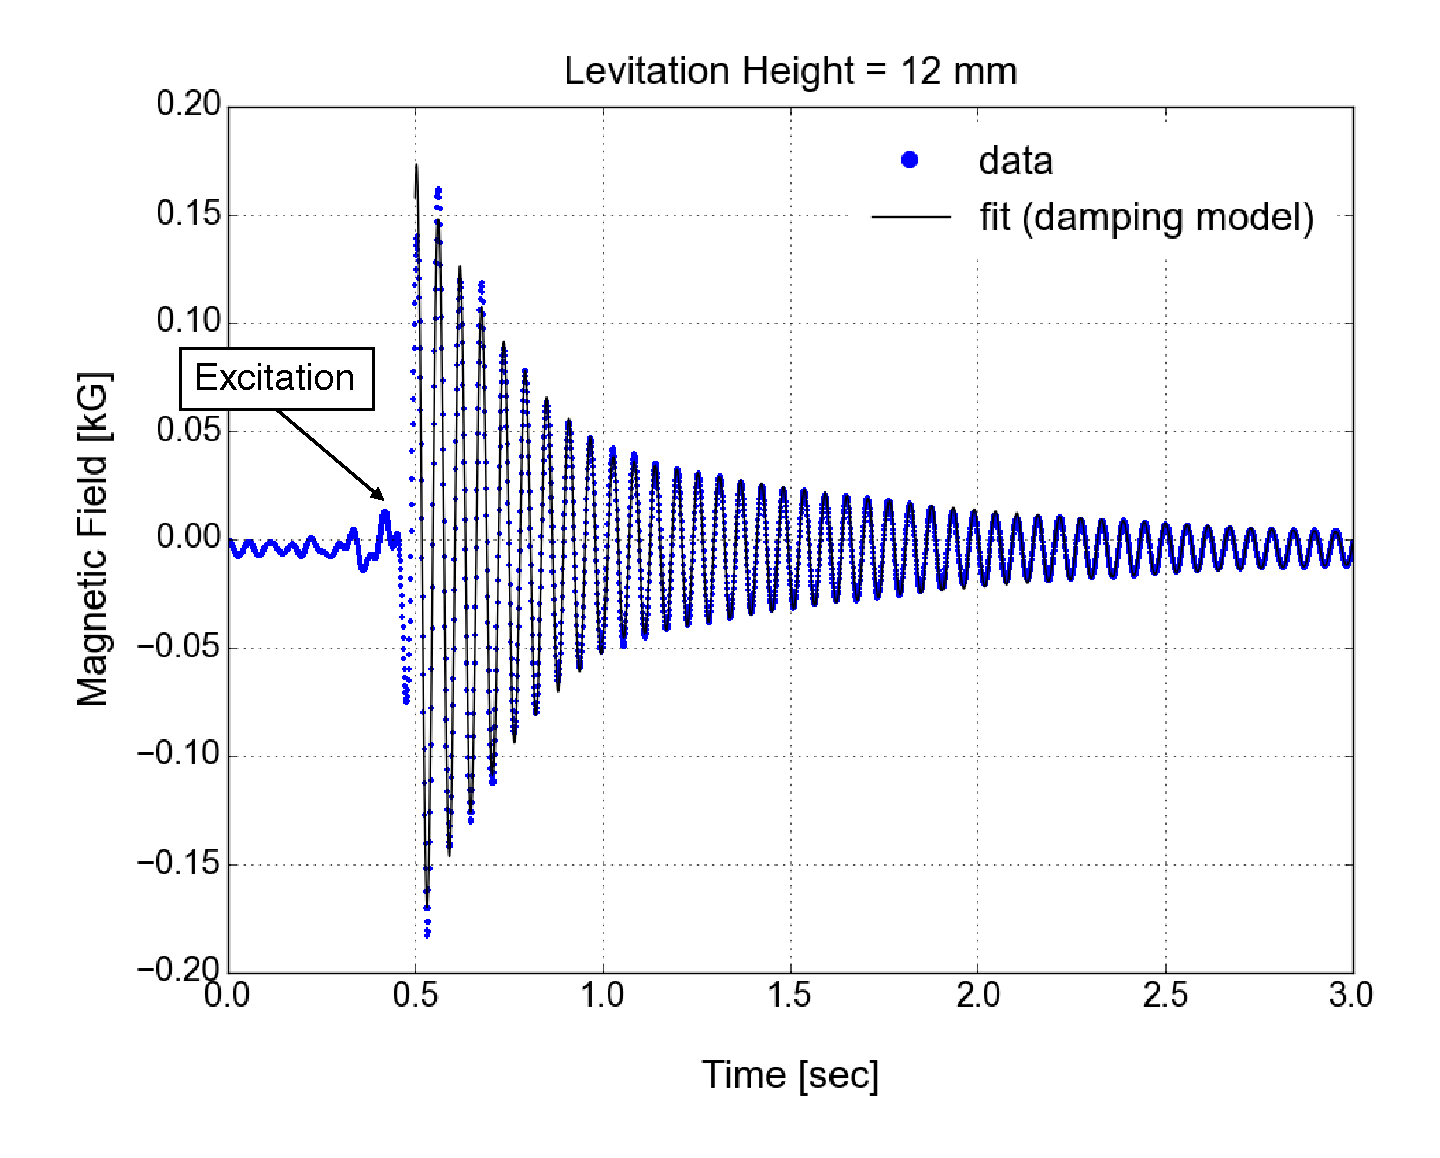
\includegraphics[width=70mm]{vibration_fit.eps}
  \end{minipage}
  \caption{The laser gauge output and the Hall sensor output as a function of time with the leviation height of 9~mm in top and bottom panels, respectivery (left).
    The fitting result of the Hall sensor output with the levitation height of 12~mm (right).}
  \label{vibration}
\end{figure}

\begin{figure}[htbp]
  \centering
  \begin{minipage}{0.45\hsize}
    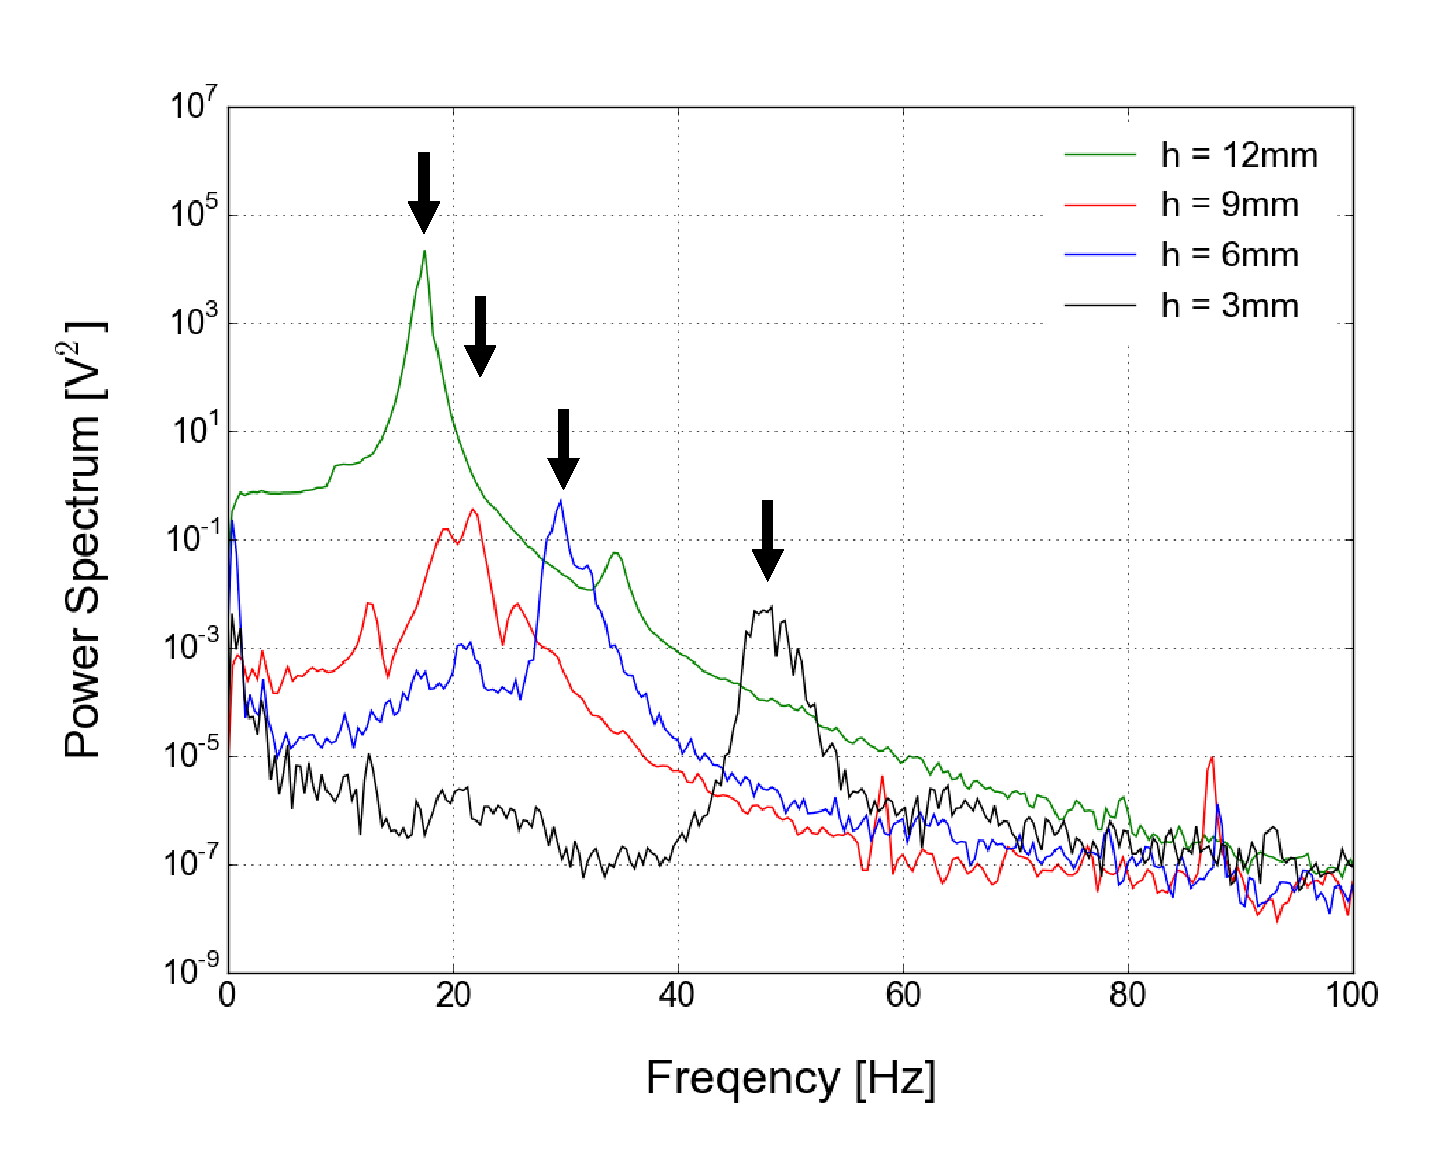
\includegraphics[width=70mm]{vibration_fft_B.eps}
  \end{minipage}
  \begin{minipage}{0.45\hsize}
    \centering
    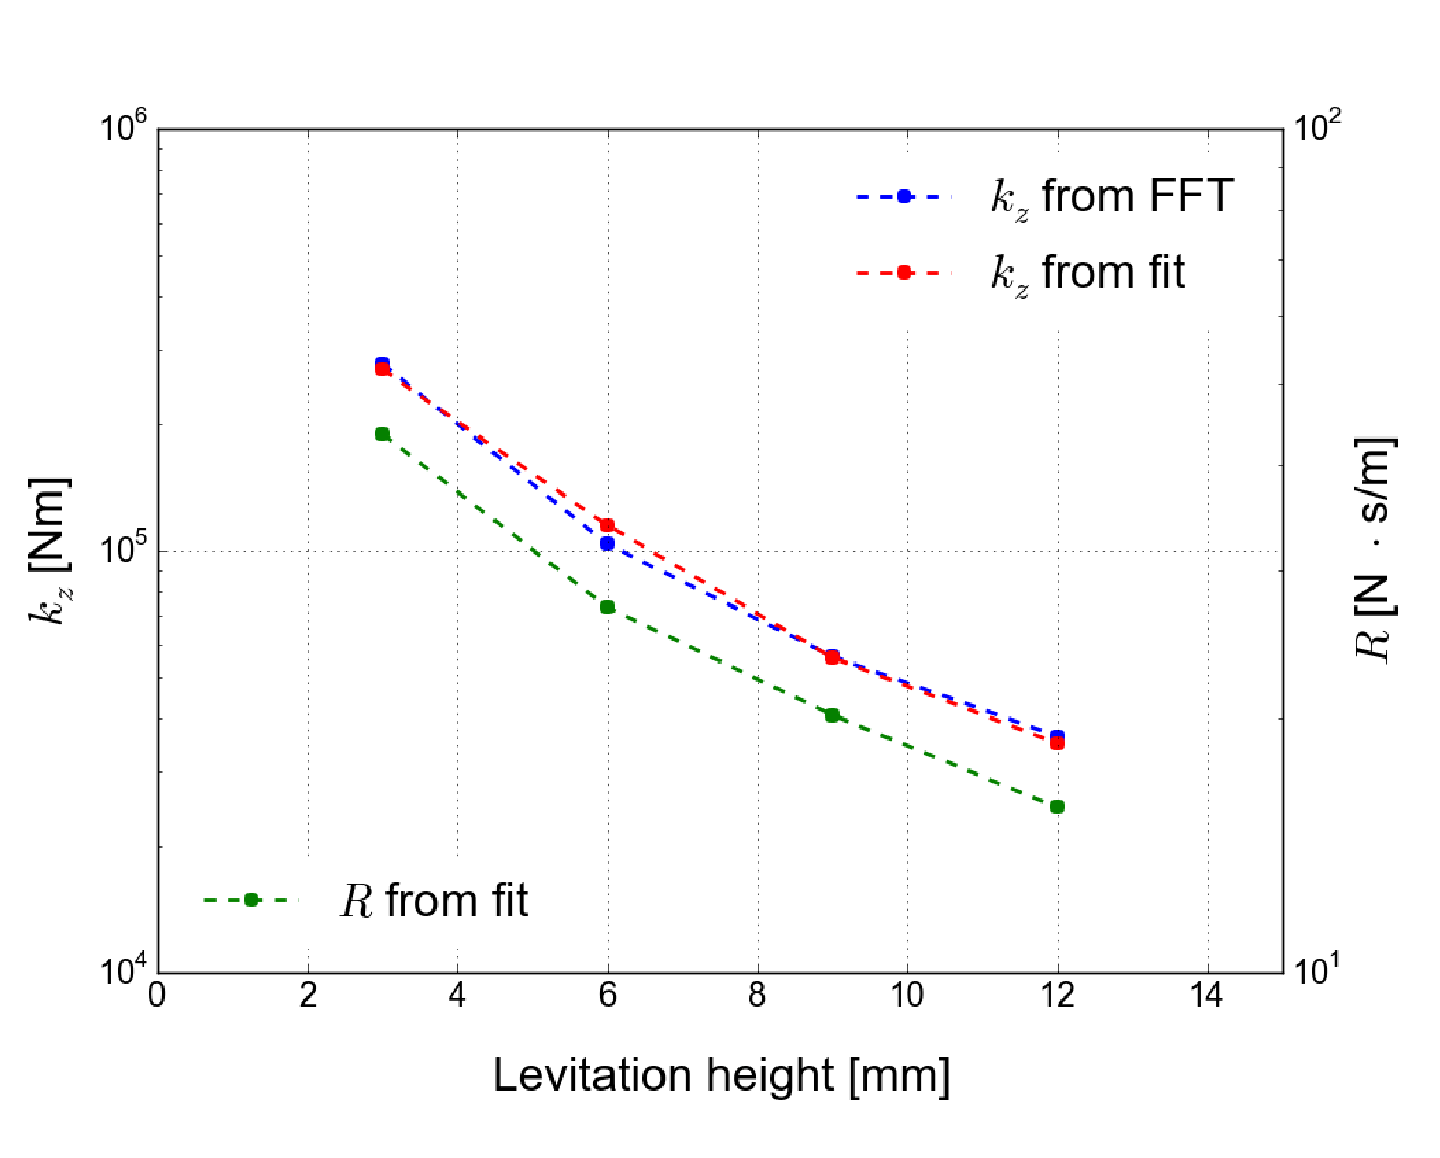
\includegraphics[width=70mm]{SpringConstant.eps}
  \end{minipage}
  \caption{The power spectrum of the Hall sensor output as a function of frequency for levitation height of 3~mm, 6~mm, 9~mm and 12~mm (left).
    The spring constant as a function of levitation heights, derived from the fit of damping model (red) and from the Fourier transformation (blue).}
  \label{fig:fft}
\end{figure}


\section*{Conclusion}
We have conducted the vibration measurements of the prototype SMB system with the diameter of $\phi$=384~mm for the polarization modulator used in CMB polarization experiments.
From the measurement, we derive the spring constant and the damping coefficient for each levitation height.
If we assume the typical mass of the HWP mounted on the rotor is $\sim$ 30~kg, the spring constant is > $10^{6}$~Nm when the levitation height is less than 6~mm.

the spring constant is in the order of $10^{4} \sim 10^{5}$~Nm and the damping coefficient is 15~45 depending on levitation height.
The increase of the spring constant is important to minimize the deviation of the HWP optical axis.
On the other hand, the increase of the damping coefficient is important to minimize the heat due to a disturbance.
As a future study, it is important to design a magnetic circuit in order to increase the spring constant and the damping coefficient.

\section*{Acknowledgment}
The author would like to thank to Dr. H. Imada at ISAS/JAXA.
This work was supported by MEXT KAKENHI Grant Numbers JP15H05441 and JSPS Core-to-Core Program, A. Advanced Research Networks.
This work was also supported by World Premier International Research Center Initiative (WPI), MEXT, Japan.


\vspace*{5mm}
\begin{thebibliography}{99}

\bibitem{inflation_sato}
 K. Sato, "First-order phase transition of a vacuum and the expansion of the Universe", Monthly Notices of Royal Astronomical Society, {\bf 195}, 467, (1981).
\bibitem{inflation_guth}
A. H. Guth, "The Inflationary Universe: A Possible Solution to the Horizon and Flatness Problems", Phys. Rev. D {\bf 23}, 347 (1981).
\bibitem{smb}
J. Hull, Topical review: Superconducting bearings, Superconductor Science, 110, 140, Technology 13 (1).
\bibitem{ebex}
J. Klein et al.,"A cryogenic half-wave plate polarimeter using a superconducting magnetic bearing," in Proc. 8th Cryogen. Opt. Syst. Instrum., San Diego, CA, USA, Aug. 2011, pp. 1–10.
\bibitem{litebird}
T. Masumura et al., "LiteBIRD: mission overview and design tradeoffs", Proc. SPIE 9143, Space Telescopes and Instrumentation 2014, 91431F, Aug. 2014.
\bibitem{matsumura_eucas2015}
T. Matsumura, H. Kataza, S. Utsunomiya, R. Yamamoto, M. Hazumi, N. Katayama, Prototype design and performance of a polarization modulator for use in space using a superconducting magnetic bearing, IEEE, TRANSACTIONS ON APPLIED SUPERCONDUCTIVITY 26 (3).
\bibitem{atz}
ATZ, http://www.atz-gmbh.com.
\end{thebibliography}


\end{document}


